\section{28. November 2018}
%! Hier gibts schon ein bisschen was hier: https://docs.google.com/document/d/1VvuRhqSy6umcpChijdMtuYw5qB0H7iJZGPXQbSMj6zA/edit
\question{Skizzieren Sie die wesentlichen Elemente der Born-Oppenheimer Näherung.}
\label{q:61}

Siehe \aqref{21}.


\question{Diskutieren Sie die sp-, sp2-, sp3-Hybridisierung in mehratomigen Molekülen.}
\label{q:62}

Hybridisierung bedeutet eine Mischung aus s- und p- Orbitalen,
hervorgerufen durch die Verformung der Elektronenhülle auf Grund
der Wechselwirkung zwischen den an der Bindung beteiligten Atomen.
Dabei gibt es die sp-, die sp2- und die sp3-Hybridisierung:

\begin{itemize}
    \item Eine sp-Hybridisierung führt zu zwei entgegengerichteten Bindungen und damit
          zu einem linearen Molekül, wenn keine anderen Bindungen vorhanden sind. Hier hybridisieren das 2s und ein 2p Orbital zu zwei sp-Orbitalen.
         
          \begin{figure}[H]
            \begin{minipage}[b]{0.5\linewidth} 
               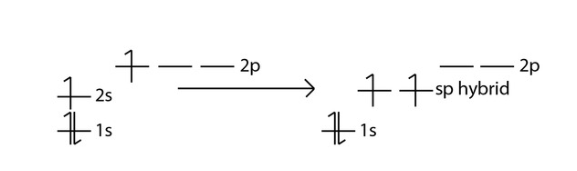
\includegraphics[width=0.8\linewidth]{resources/28-11-2018/sp11.PNG}
               \caption{sp-Hybridisierung, wobei die Energie sinkt}
            \end{minipage}
            \hspace{0.01\linewidth}
            \begin{minipage}[b]{0.5\linewidth} 
               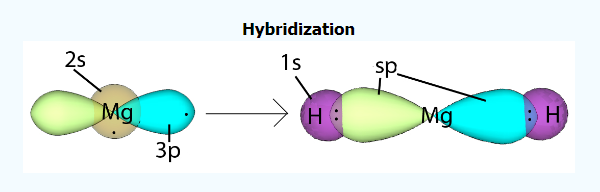
\includegraphics[width=0.8\linewidth]{resources/28-11-2018/sp12.PNG}
               \caption{sp-Hybridisierung am Beispiel von Magnesium }
            \end{minipage}
         \end{figure}

    \item Die sp2-Hybridisierung führt zu drei gerichteten Bindungen, die in einer
          Ebene liegen. Hier bilden sich aus den 2s und zwei 2p-Orbitalen, drei sp-Orbitale.

          \begin{figure}[H]
            \begin{minipage}[b]{0.5\linewidth} 
               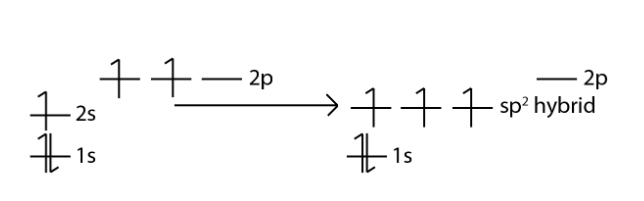
\includegraphics[width=0.8\linewidth]{resources/28-11-2018/sp21.PNG}
               \caption{sp2-Hybridisierung, wobei die Energie sinkt}
            \end{minipage}
            \hspace{0.01\linewidth}
            \begin{minipage}[b]{0.5\linewidth} 
               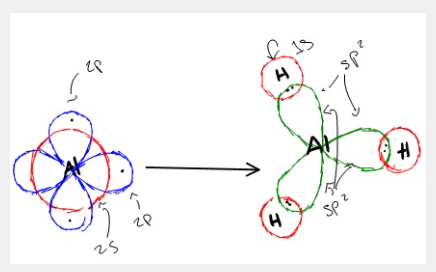
\includegraphics[width=0.8\linewidth]{resources/28-11-2018/sp22.PNG}
               \caption{sp2-Hybridisierung am Beispiel von Aluminiumhydroxid}
            \end{minipage}
         \end{figure}

    \item Für die sp3-Hybridisierung ergeben sich Atomorbitale mit Maxima, die in die vier Ecken eines Tetraeders zeigen.
          Hier bilden sich aus den 2s und drei 2p-Orbitalen, vier sp3-Orbitale.

          \begin{figure}[H]
            \begin{minipage}[b]{0.5\linewidth} 
               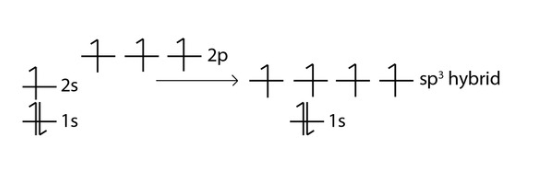
\includegraphics[width=0.8\linewidth]{resources/28-11-2018/sp31.PNG}
               \caption{sp3-Hybridisierung, wobei die Energie sinkt}
            \end{minipage}
            \hspace{0.01\linewidth}
            \begin{minipage}[b]{0.5\linewidth} 
               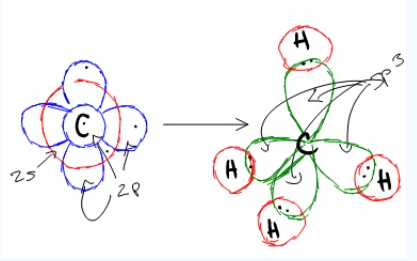
\includegraphics[width=0.8\linewidth]{resources/28-11-2018/sp32.PNG}
               \caption{sp3-Hybridisierung am Beispiel von Methan}
            \end{minipage}
         \end{figure}

\end{itemize}

\question{Diskutieren Sie die Laue'sche Beugungsbedingung anhand der Ewald-Konstruktion im Rahmen der Bragg'schen Interpretation.}
\label{q:63}

\question{Wodurch unterscheiden sich ein fcc-Gitter von einer hcp-Struktur?}
\label{q:64}

siehe \aqref{46}

\question{Diskutieren Sie die Gitterenergie der Ionenkristalle.}
\label{q:65}

\question{Vergleichen Sie die Einstein- und Debye-Modelle der spezifischen Wärme. Welche Annahmen sind in beiden Modellen zu einfach?}
\label{q:66}

\question{Diskutieren Sie das Auftreten einer Energiebandlücke mit Hilfe des Modells der fast freien Elektronen.}
\label{q:67}

siehe \aqref{5}

\question{Wodurch unterscheidet sich die Dispersionsrelation der Phononen eines primitiven kubischen Gitters von jenem eines CsCl-Gitters.}
\label{q:68}

\question{Erklären Sie die chemische Bindung von \ch{O2} ($Z=8$).}
\label{q:69}

\[\ch{O2} : (1\sigma_g)^2 ~ (1\sigma_u^*)^2 ~ (2\sigma_g)^2 ~ (2\sigma_u^*)^2 ~ (3\sigma_g)^2 ~ (1\pi_g)^4 ~ (1\pi_u^*)^2\]

Da beide Sauerstoffatome je zwei freie Valenzelektronen haben, kommt es zu einer Doppelbindung.

\setcapindent{0pt}
\begin{figure}[H]
   \centering
   \begin{minipage}[t]{0.475\linewidth}
      \centering
      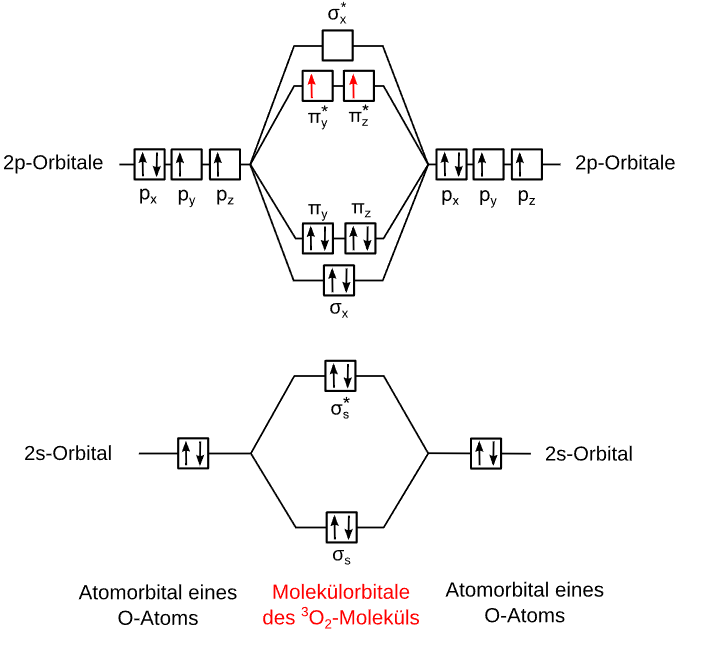
\includegraphics[width=\linewidth]{resources/28-11-2018/O2.PNG}
      \caption{Elektronenkonfiguration von \ch{O2}}
      \label{fig:Elektronenkonfiguration_O2}
   \end{minipage}%
   \hspace*{\fill}
   \begin{minipage}[t]{0.475\linewidth}
      \centering
      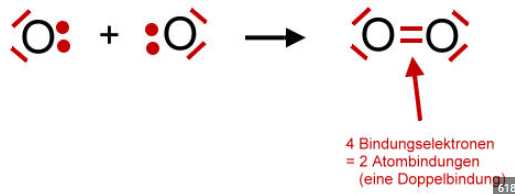
\includegraphics[width=\linewidth]{resources/28-11-2018/o2_bindung.PNG}
      \caption{Chemische Bindung zweier Sauerstoffatome}
      \label{fig:chemische_Bindung_O2}
   \end{minipage}
\end{figure}
\setcaphanging

\newpage